% =========================================================================
% CAPITOLO 2: DATASET (SPOTIFY)
% =========================================================================
\section{Spotify tracks analysis: dataset}

Il dataset impiegato per la realizzazione di questo progetto è stato reperito dalla piattaforma Kaggle, ed è noto come \textit{Spotify Audio Features / Genres v2}. Il dataset grezzo raccoglie \textbf{42.305 osservazioni} relative a brani musicali estratti tramite le Web API ufficiali di Spotify a partire da playlist pubbliche focalizzate su \textbf{15 generi e sottogeneri} musicali contemporanei. 

Ciascuna traccia all'interno del dataset è descritta da un totale di \textbf{22 attributi}, comprendenti metadati identificativi, parametri sonori continui derivati dall'analisi spettrale e variabili discrete legate alla teoria musicale. Nel dettaglio, le informazioni fornite dal dataset si suddividono nelle seguenti categorie:

\begin{itemize}
    \item \textbf{Informazioni e metadati di servizio:}
    \begin{itemize}
        \item \texttt{id}: Stringa alfanumerica univoca assegnata da Spotify a ciascun brano.
        \item \texttt{song\_name} e \texttt{title}: Titolo della traccia o stringa del nome del file.
        \item \texttt{uri}, \texttt{track\_href}, \texttt{analysis\_url}: Indirizzi URI e URL web per l'accesso programmatico alle risorse audio sui server di Spotify.
        \item \texttt{type}: Tipologia dell'oggetto ritornato dall'API (pari ad \texttt{audio\_features}).
        \item \texttt{genre}: Genere musicale associato alla playlist da cui è stato estratto il brano (rappresenta la nostra variabile target per la classificazione).
    \end{itemize}
    \item \textbf{Caratteristiche audio continue (misure fisiche e psicoacustiche):}
    \begin{itemize}
        \item \texttt{danceability}: Valore compreso tra 0.0 e 1.0 che descrive quanto un brano sia adatto al ballo, calcolato sulla base di regolarità del ritmo, stabilità del tempo e forza della battuta.
        \item \texttt{energy}: Valore tra 0.0 e 1.0 che rappresenta una misura percettiva dell'intensità e dell'attività della traccia (i brani energici risultano veloci, rumorosi e densi).
        \item \texttt{loudness}: Volume sonoro complessivo della traccia espresso in decibel (dB), tipicamente compreso tra -60 dB e 0 dB.
        \item \texttt{speechiness}: Valore tra 0.0 e 1.0 che quantifica la presenza di parole parlate. Valori superiori a 0.66 indicano tracce parlate (es. talk show o poesia), valori tra 0.33 e 0.66 indicano musica con forte presenza vocale ritmata (Rap, Trap), mentre valori inferiori a 0.33 descrivono brani tradizionali e strumentali.
        \item \texttt{acousticness}: Misura di confidenza tra 0.0 e 1.0 che indica se il brano è acustico (1.0) o sintetico/elettronico (vicino a 0.0).
        \item \texttt{instrumentalness}: Valore tra 0.0 e 1.0 che prevede se la traccia è priva di parti vocali cantate. I brani rap o pop ottengono valori prossimi a 0, mentre tracce techno o ambient superano 0.5.
        \item \texttt{liveness}: Valore tra 0.0 e 1.0 che rileva la presenza di un pubblico nella registrazione; valori superiori a 0.8 indicano un'alta probabilità di performance dal vivo.
        \item \texttt{valence}: Valore da 0.0 a 1.0 che descrive la positività musicale trasmessa dalla traccia: valori alti indicano euforia, allegria e serenità, mentre valori bassi denotano tristezza, rabbia o tensione emotiva.
        \item \texttt{tempo}: Velocità stimata del brano espressa in battiti al minuto (BPM).
        \item \texttt{duration\_ms}: Durata temporale complessiva del brano espressa in millisecondi.
    \end{itemize}
    \item \textbf{Parametri musicali discreti:}
    \begin{itemize}
        \item \texttt{key}: Tonalità complessiva del brano codificata come intero secondo la notazione standard Pitch Class (0 = Do, 1 = Do$\sharp$/Re$\flat$, 2 = Re, ..., 11 = Si).
        \item \texttt{mode}: Modalità del brano, dove 1 indica la modalità Maggiore e 0 indica la modalità Minore.
        \item \texttt{time\_signature}: Metro ritmico stimato (numero di quarti per battuta, tipicamente pari a 4 nella quasi totalità della musica moderna).
    \end{itemize}
\end{itemize}

Nella Tabella \ref{tab:colonne_dataset} vediamo una rappresentazione riepilogativa delle colonne del dataset e il relativo formato dei dati.

\begin{table}[H]
\centering
\caption{Colonne del dataset e relativo formato dei dati.}
\label{tab:colonne_dataset}
\vspace{0.2cm}
\begin{tabular}{lll}
\toprule
\textbf{Colonna} & \textbf{Formato} & \textbf{Descrizione / Range} \\
\midrule
\texttt{danceability} & Float & Ballabilità del brano [0.0 - 1.0] \\
\texttt{energy} & Float & Intensità dinamica percepita [0.0 - 1.0] \\
\texttt{key} & Intero & Tonalità Pitch Class [0 - 11] \\
\texttt{loudness} & Float & Volume globale in decibel [dB] \\
\texttt{mode} & Intero & Modalità armonica [0 = Minore, 1 = Maggiore] \\
\texttt{speechiness} & Float & Presenza di parlato / flow vocale [0.0 - 1.0] \\
\texttt{acousticness} & Float & Grado di produzione acustica [0.0 - 1.0] \\
\texttt{instrumentalness} & Float & Assenza di parti vocali [0.0 - 1.0] \\
\texttt{liveness} & Float & Presenza di registrazione live [0.0 - 1.0] \\
\texttt{valence} & Float & Positività / Tonalità emotiva [0.0 - 1.0] \\
\texttt{tempo} & Float & Velocità ritmica in BPM \\
\texttt{duration\_ms} & Intero & Durata del brano in millisecondi \\
\texttt{time\_signature} & Intero & Metro ritmico stimato [3 - 5] \\
\texttt{id} & Stringa & Identificativo univoco Spotify \\
\texttt{genre} & Categoriale & Etichetta del genere (15 classi target) \\
\bottomrule
\end{tabular}
\end{table}

\newpage
\subsection{ETL}

Il processo di ETL (Extract, Transform, Load) è stato un passaggio fondamentale per garantire la qualità dei dati e la validità scientifica di tutte le analisi condotte successivamente. L'estrazione da API di playlist eterogenee, se non adeguatamente filtrata, introduce infatti distorsioni sistematiche che possono compromettere l'addestramento dei modelli.

Durante questa fase sono state applicate diverse operazioni critiche:

\begin{itemize}
    \item \textbf{Deduplicazione su Track ID:} Poiché le playlist Spotify condividono spesso brani popolari comuni a più sottogeneri, il dataset grezzo originale di 42.305 righe presentava un elevato numero di repliche dello stesso brano. È stato eseguito un filtraggio rigoroso basato sulla colonna \texttt{id}, individuando e rimuovendo esattamente \textbf{6.428 record duplicati}. Il dataset ripulito risulta così composto da \textbf{35.877 brani unici effettivi}. 
    Questa operazione si è rivelata indispensabile: in assenza di deduplicazione preventiva, brani identici sarebbero finiti contemporaneamente sia nel training set che nel test set durante la fase di holdout, provocando un grave fenomeno di \textit{data leakage} e generando stime di accuratezza artificialmente gonfiate e non generalizzabili.
    
    \item \textbf{Eliminazione delle Variabili di Servizio:} Sono state eliminate tutte le colonne prive di contenuto acustico utile alla modellazione predittiva, tra cui \texttt{Unnamed: 0}, \texttt{type}, \texttt{uri}, \texttt{track\_href}, \texttt{analysis\_url}, \texttt{song\_name} e \texttt{title}. Oltre a non apportare informazione sonica, tali variabili avrebbero appesantito la memoria computazionale introducendo rumore inutile.
    
    \item \textbf{Verifica dell'Integrità e Gestione dei Valori Nulli:} È stato effettuato un controllo esaustivo per rilevare l'eventuale presenza di valori nulli o mancanti (\textit{missing values}). Tutte le feature audio numeriche e la variabile target \texttt{genre} risultano complete al 100\%, confermando l'assenza di dati mancanti da imputare.
    
    \item \textbf{Esportazione del Dataset Pulito:} Il dataset risultante dalle operazioni di ETL è stato salvato nel file \texttt{genres\_cleaned.csv}, pronto per essere utilizzato in modo riproducibile dalle pipeline di analisi descrittiva, classificazione e clustering.
\end{itemize}

\newpage
\subsection{Analisi descrittiva}

L'analisi descrittiva ha avuto lo scopo di esplorare e sintetizzare le principali caratteristiche statistiche del dataset, fornendo una comprensione preliminare delle distribuzioni marginali delle variabili e delle relazioni che intercorrono tra di esse. Nel seguito vengono esaminate singolarmente le distribuzioni dei generi, delle feature continue, delle grandezze musicali discrete e la matrice di correlazione.

\subsubsection{Distribuzione dei generi musicali}

La frequenza con cui ciascun genere musicale compare all'interno del dataset ripulito è stata visualizzata tramite il grafico a barre riportato in Figura \ref{fig:distribuzione_generi}. 

\begin{figure}[H]
    \centering
    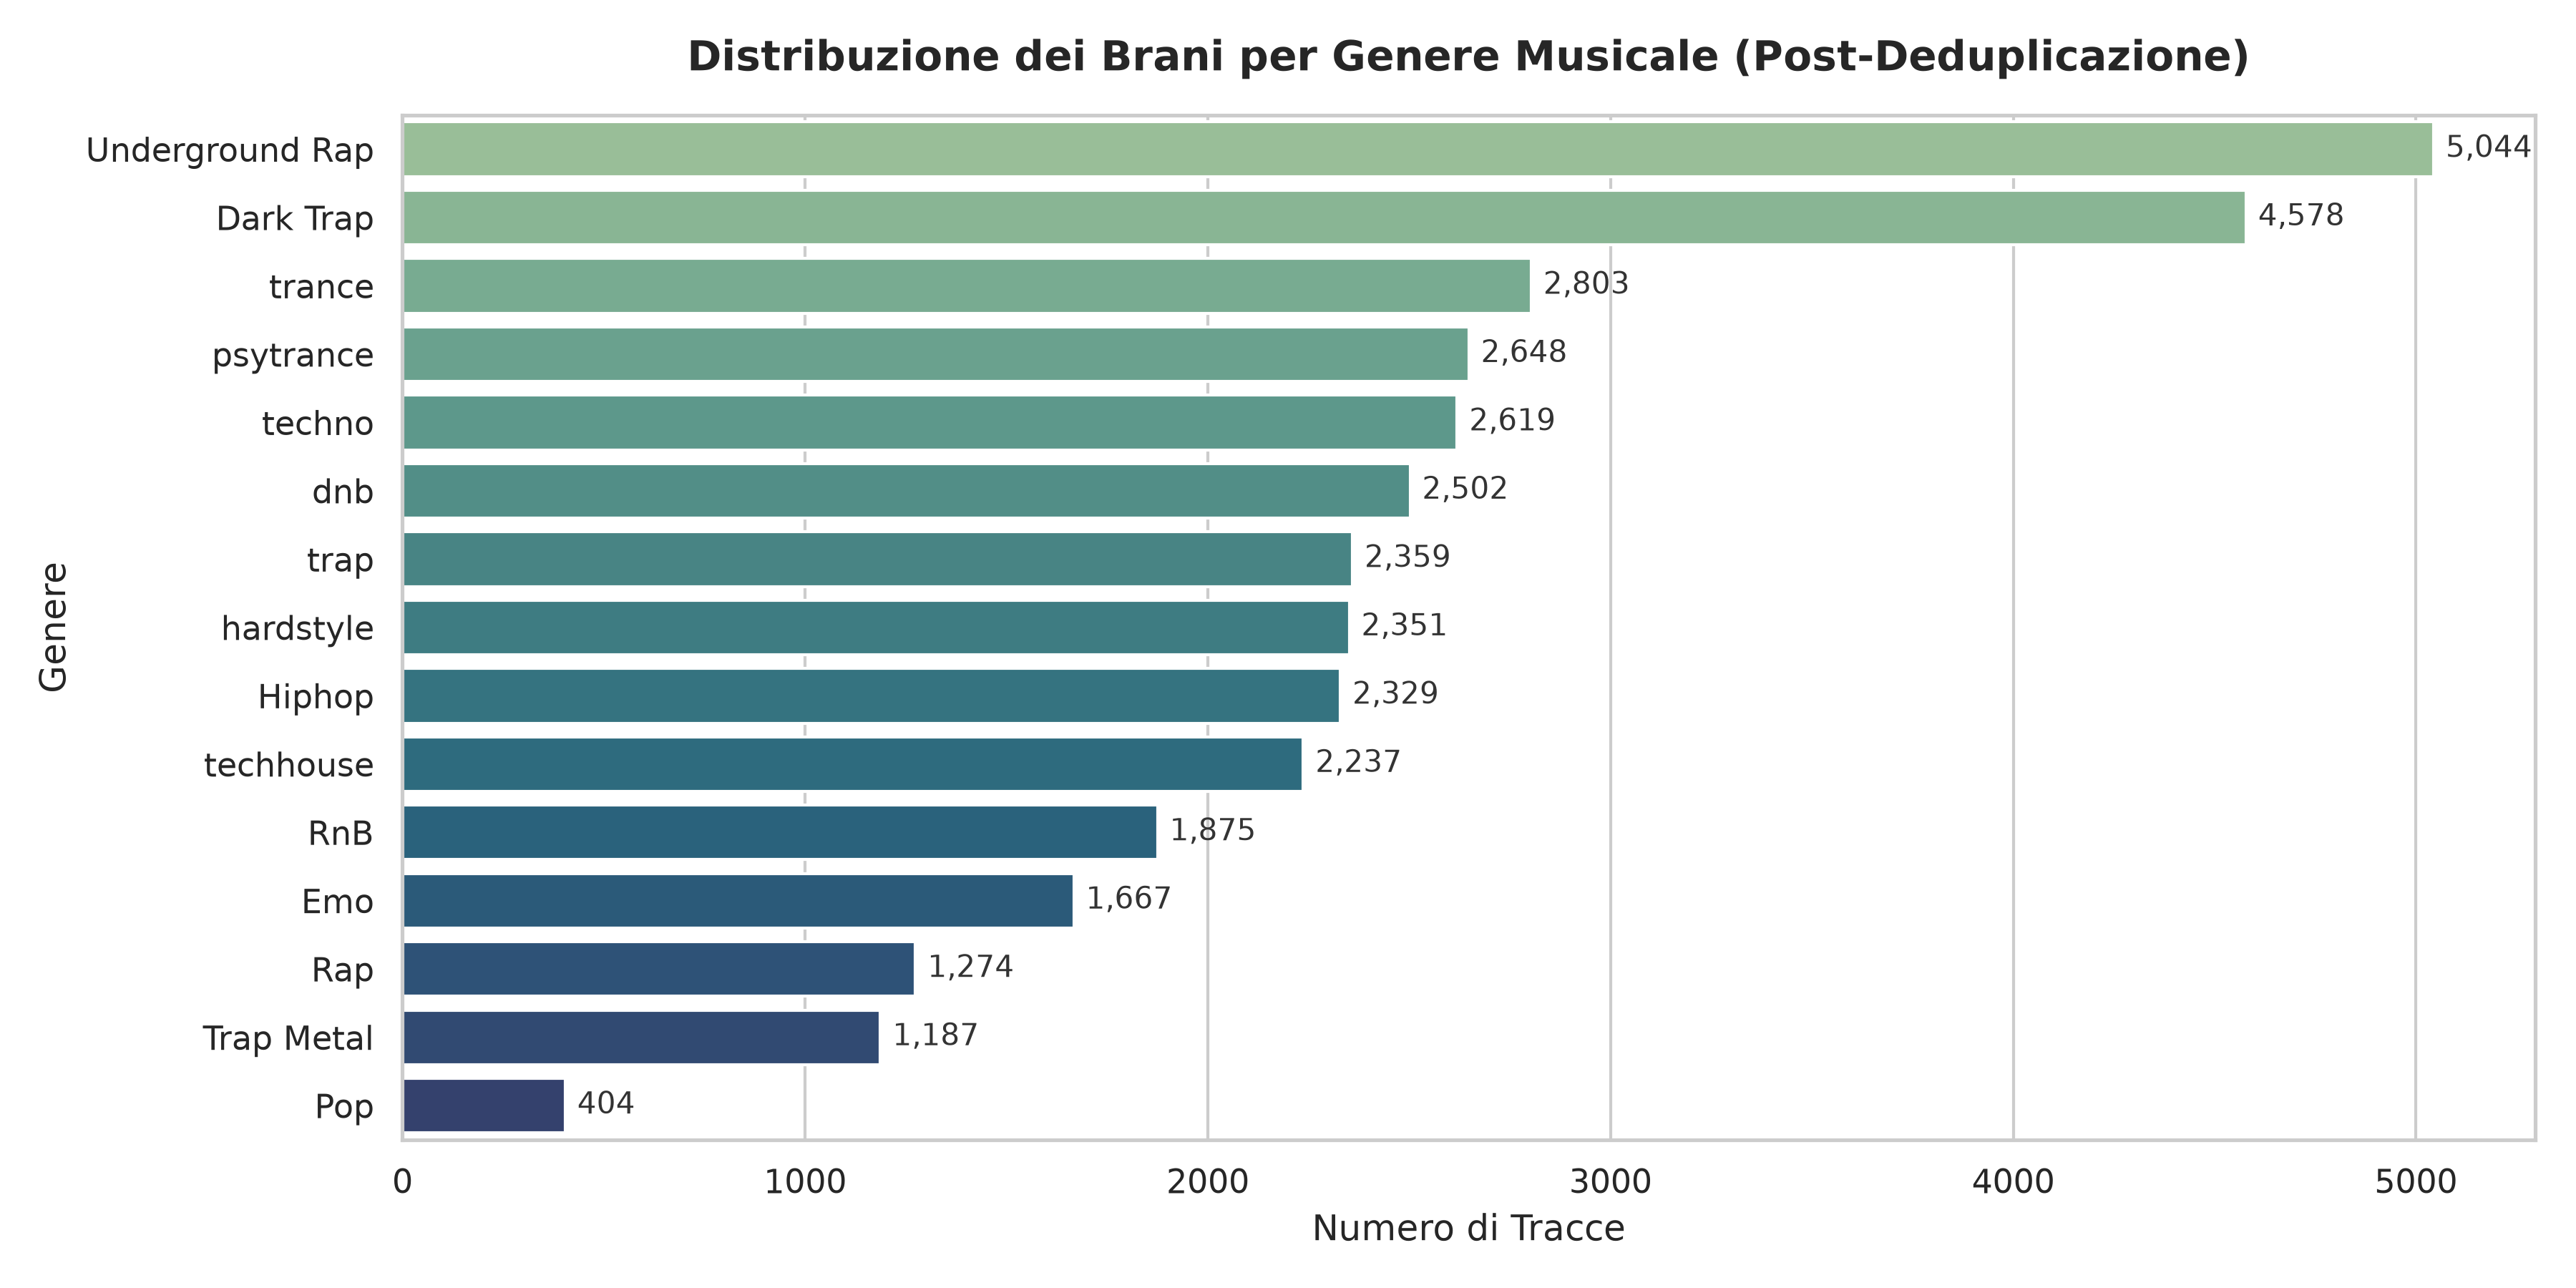
\includegraphics[width=0.88\textwidth]{capitolo2/img/fig01_distribuzione_generi.png}
    \caption{Distribuzione delle frequenze dei 15 generi musicali nel dataset post-ETL.}
    \label{fig:distribuzione_generi}
\end{figure}

Come si può osservare chiaramente dalla Figura \ref{fig:distribuzione_generi}, il dataset evidenzia un marcato sbilanciamento naturale nella numerosità delle classi. I generi urbani ed elettronici risultano ampiamente dominanti: in particolare, \textit{Underground Rap} conta 5.044 brani e \textit{Dark Trap} ne conta 4.578. Al contrario, altri generi risultano fortemente sottorappresentati: il caso più evidente è il genere \textit{Pop}, che include appena 404 brani, seguito da \textit{Rap} (1.042) ed \textit{Emo} (1.616). 

Questo squilibrio rappresenta una seria criticità per i successivi modelli di classificazione: un algoritmo addestrato ingenuamente su queste proporzioni tenderebbe infatti a favorire sistematicamente le classi maggioritarie, sacrificando l'accuratezza sulle classi rare. Tale evidenza ha reso indispensabile la successiva adozione di strategie di ricampionamento bilanciato.

\newpage
\subsubsection{Distribuzione delle feature continue}

Per analizzare le variabili numeriche continue, sono stati generati istogrammi affiancati dalle relative curve di densità stimate tramite Kernel Density Estimation (KDE), riportati complessivamente in Figura \ref{fig:audio_features_hist}.

\begin{figure}[H]
    \centering
    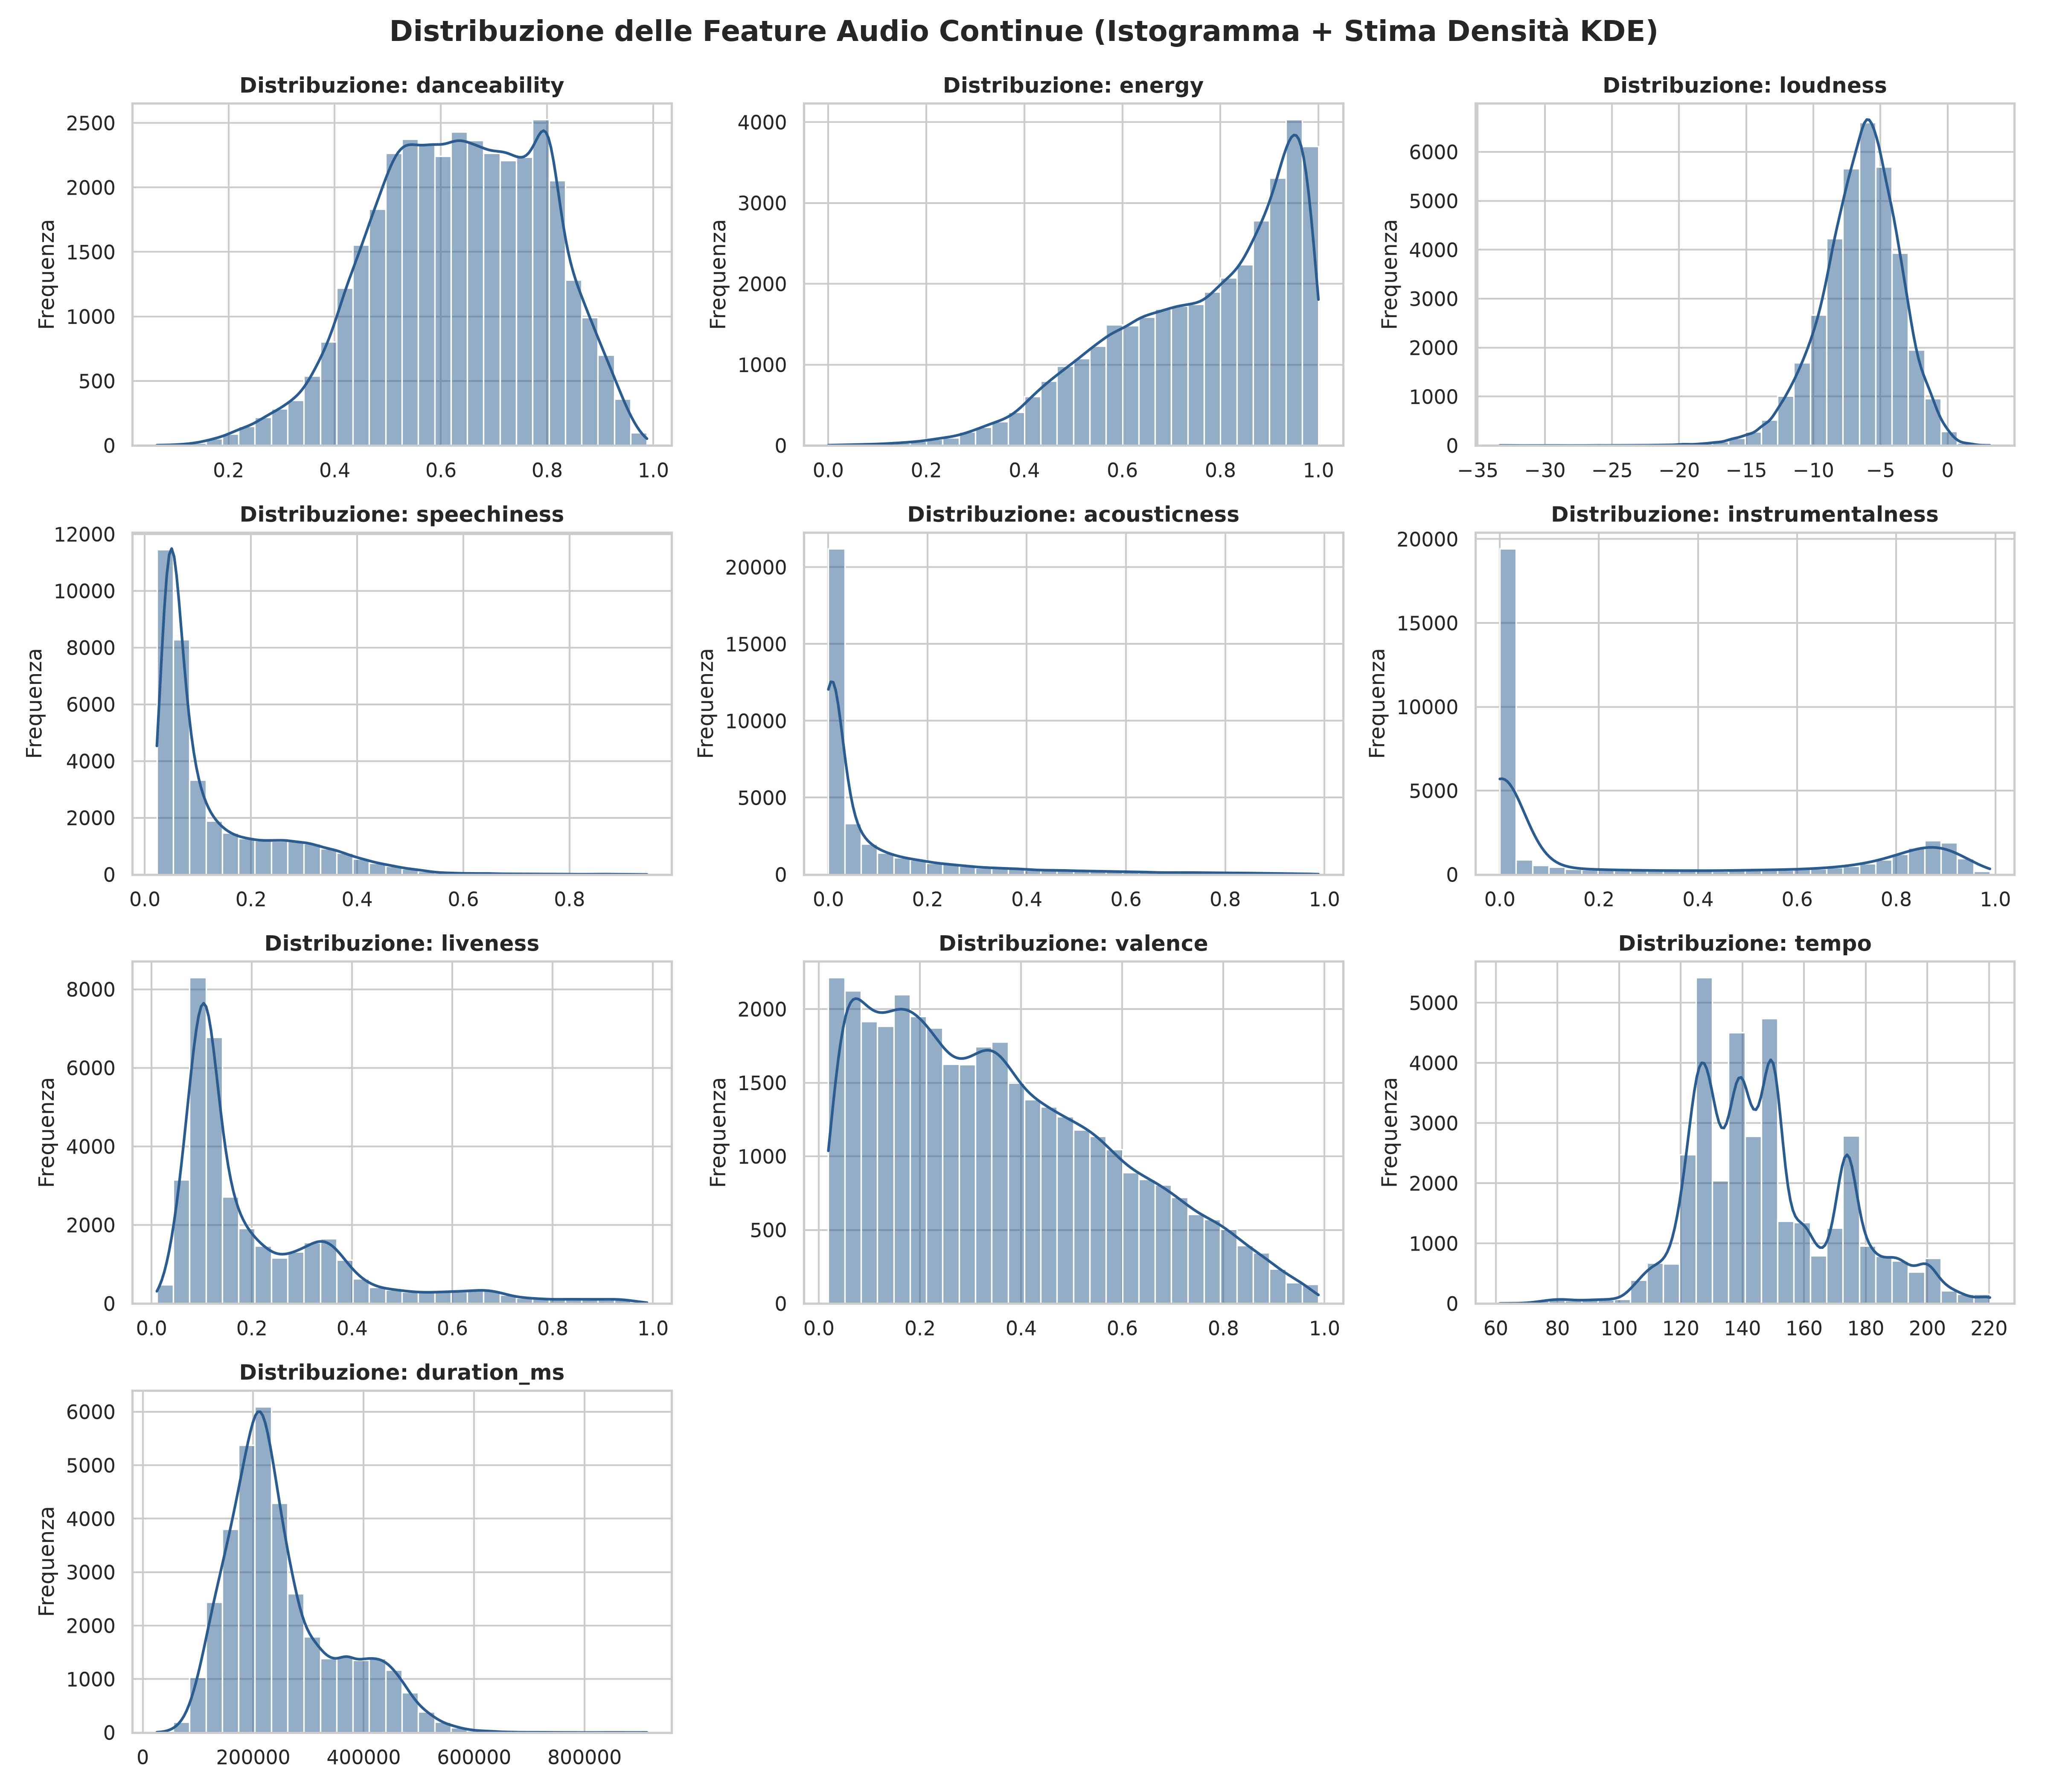
\includegraphics[width=0.92\textwidth]{capitolo2/img/fig02_audio_features_hist_kde.png}
    \caption{Distribuzione delle caratteristiche audio continue (istogrammi e curve di densità KDE).}
    \label{fig:audio_features_hist}
\end{figure}

Dall'ispezione della Figura \ref{fig:audio_features_hist} emergono interessanti pattern acustici e produttivi:
\begin{itemize}
    \item \texttt{danceability}: Mostra una distribuzione quasi perfettamente simmetrica e a campana, con una media centrata tra 0.65 e 0.70. Questo riflette il fatto che la maggior parte delle tracce campionate appartiene a generi pensati per l'ascolto ritmico e il ballo.
    \item \texttt{energy} e \texttt{loudness}: Presentano entrambe una marcata asimmetria negativa (coda allungata verso sinistra). La quasi totalità dei brani presenta valori di energia superiori a 0.6 e volumi compresi tra -8 dB e -4 dB. Questo fenomeno è una conseguenza diretta delle moderne tecniche di mastering discografico (la cosiddetta \textit{loudness war}), che tendono a massimizzare la percezione di impatto sonoro riducendo la gamma dinamica.
    \item \texttt{acousticness}: Mostra un picco estremamente pronunciato in prossimità dello zero, a testimonianza del fatto che i generi presenti nel dataset fanno un uso massiccio di strumenti sintetici, campionatori e drum machine elettroniche.
    \item \texttt{speechiness}: Mostra una struttura bimodale caratteristica: un primo gruppo preponderante si addensa al di sotto di 0.1 (brani melodici o strumentali tradizionali), mentre una seconda gobba ben definita compare oltre 0.25, tipica delle tracce rap e trap caratterizzate da un denso flusso vocale ritmato.
    \item \texttt{tempo}: È distribuito principalmente tra 70 e 190 BPM, con addensamenti visibili in corrispondenza delle convenzioni di genere standard (130-140 BPM per trap ed EDM, 170-175 BPM per drum and bass).
\end{itemize}

\newpage
\subsubsection{Distribuzione delle variabili discrete}

La Figura \ref{fig:discrete_features} riporta la distribuzione di frequenza per le tre grandezze discrete legate alla teoria musicale: la tonalità (\texttt{key}), la modalità (\texttt{mode}) e la divisione metrica (\texttt{time\_signature}).

\begin{figure}[H]
    \centering
    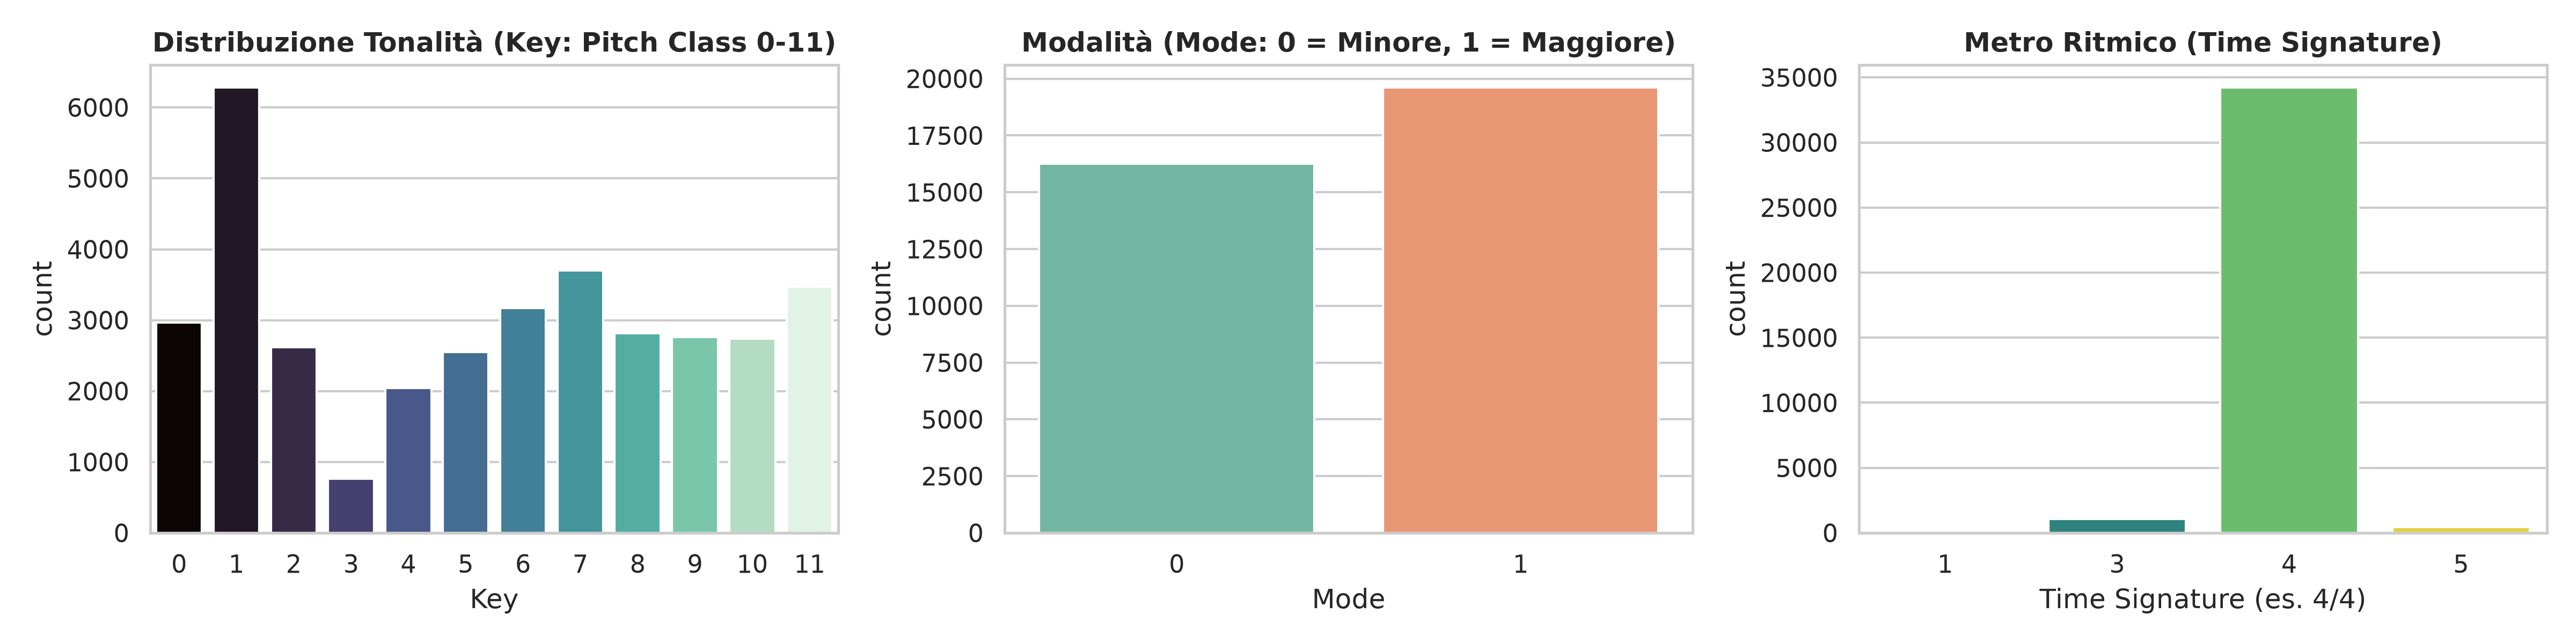
\includegraphics[width=0.90\textwidth]{capitolo2/img/fig03_discrete_features.png}
    \caption{Distribuzione delle variabili discrete: Tonalità (\texttt{key}), Modo (\texttt{mode}) e Metro (\texttt{time\_signature}).}
    \label{fig:discrete_features}
\end{figure}

Dalla Figura \ref{fig:discrete_features} si evince che:
\begin{itemize}
    \item La variabile \texttt{time\_signature} vede la quasi totalità assoluta delle osservazioni concentrata sul valore 4 (ossia la misura standard in quattro quarti 4/4), comune a oltre il 95\% delle produzioni musicali contemporanee occidentali.
    \item La variabile \texttt{mode} mostra una leggera prevalenza della modalità maggiore (\texttt{mode} = 1, circa il 55\% dei brani) rispetto a quella minore (\texttt{mode} = 0, circa il 45\%), riflettendo una discreta varietà armonica.
    \item La variabile \texttt{key} si distribuisce su tutte le 12 classi di altezza (da 0 per il Do fino a 11 per il Si), con frequenze leggermente più elevate in corrispondenza di Do (0), Do$\sharp$/Re$\flat$ (1) e Sol (7), tonalità storicamente molto impiegate nella composizione di musica elettronica e urbana.
\end{itemize}

\newpage
\subsubsection{Matrice di correlazione}

Per studiare le relazioni di interdipendenza lineare tra tutte le variabili numeriche, è stata calcolata la matrice di correlazione di Pearson, visualizzata sotto forma di heatmap in Figura \ref{fig:matrice_corr_iniziale}.

\begin{figure}[H]
    \centering
    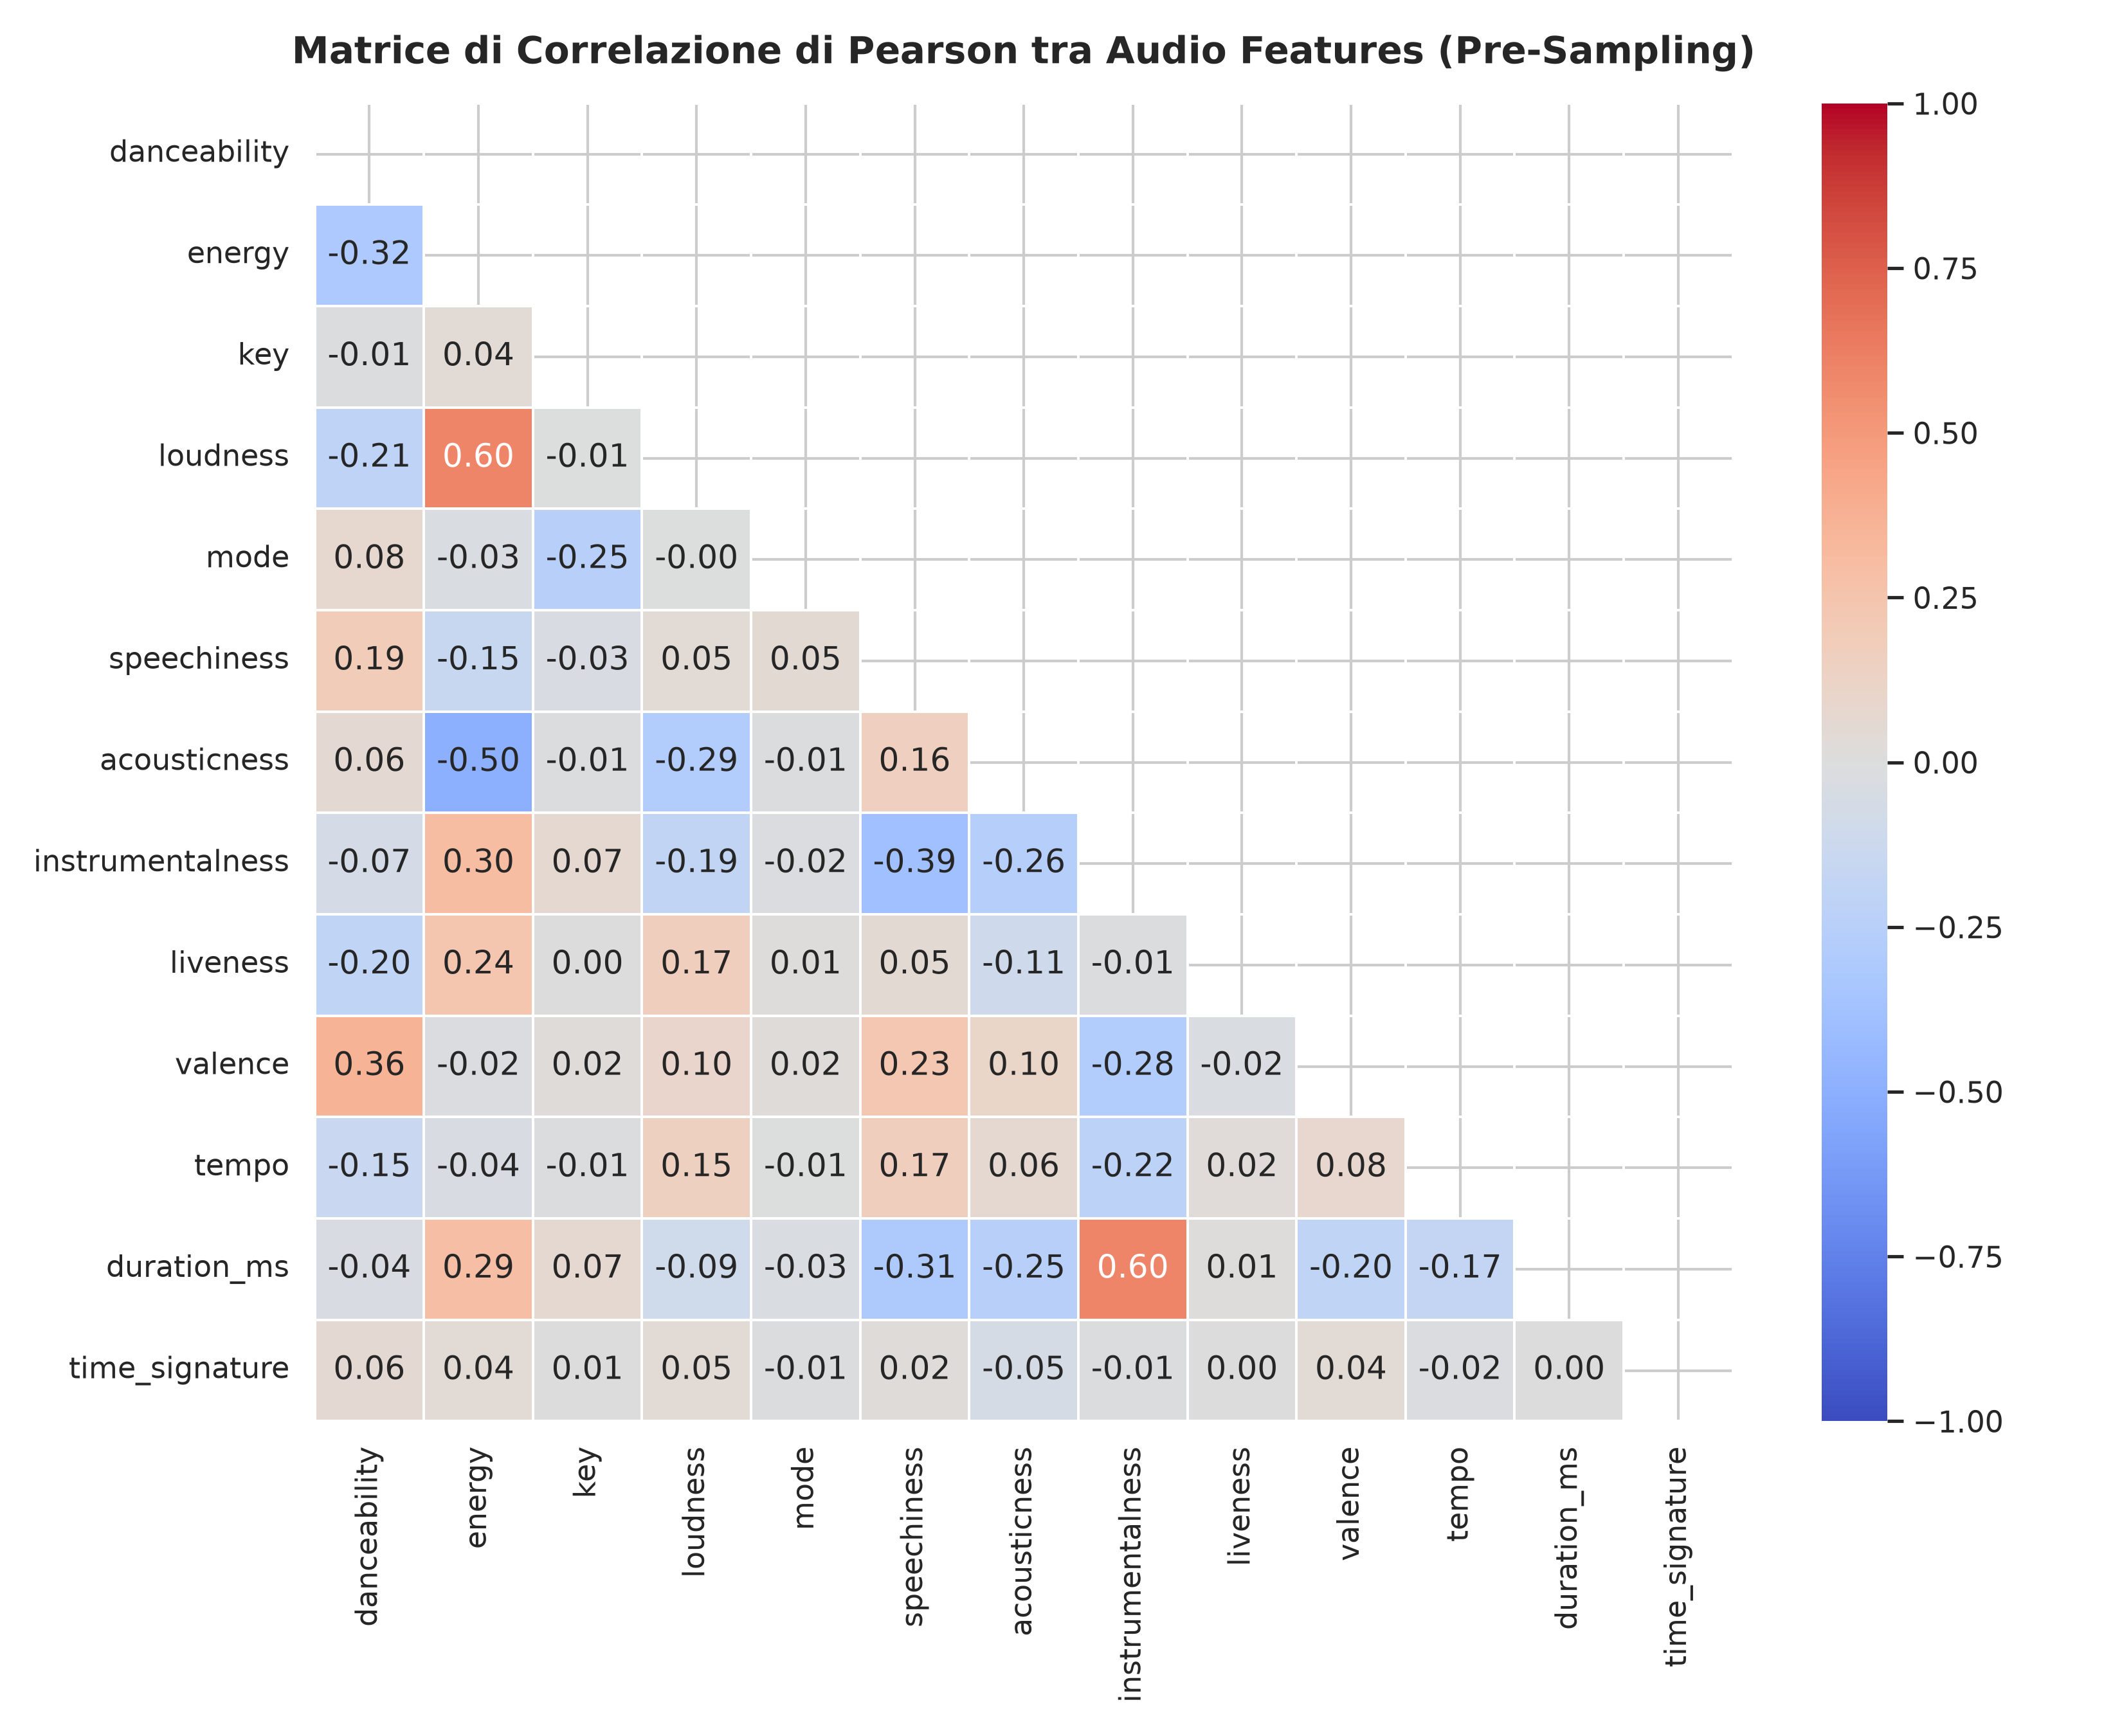
\includegraphics[width=0.78\textwidth]{capitolo2/img/fig04_matrice_correlazione_iniziale.png}
    \caption{Matrice di correlazione di Pearson tra le feature audio calcolata sul dataset prima del sampling.}
    \label{fig:matrice_corr_iniziale}
\end{figure}

Dall'analisi della Figura \ref{fig:matrice_corr_iniziale} emergono alcune correlazioni forti e perfettamente coerenti con la fisica acustica e la produzione musicale:
\begin{itemize}
    \item \textbf{Forte correlazione positiva tra \texttt{energy} e \texttt{loudness} ($r \approx 0.70$):} Brani con elevata energia dinamica presentano naturalmente livelli sonori medi più alti in decibel.
    \item \textbf{Marcata correlazione negativa tra \texttt{energy} e \texttt{acousticness} ($r \approx -0.49$):} Tracce acustiche tendono ad avere un'energia percepita significativamente inferiore rispetto a produzioni sintetiche o distorte.
    \item \textbf{Correlazione positiva moderata tra \texttt{valence} e \texttt{danceability} ($r \approx 0.35$):} I brani dal tono emotivo più allegro ed euforico sono tendenzialmente più facili da ballare rispetto a brani malinconici o tesi.
    \item \textbf{Quasi totale indipendenza di \texttt{duration\_ms} e \texttt{key}:} Queste variabili presentano coefficienti prossimi a 0 rispetto alla maggior parte delle altre grandezze, indicando che la tonalità o la lunghezza del brano non vincolano direttamente l'energia o la ballabilità.
\end{itemize}

